\documentclass{bioinfo}


\copyrightyear{2010}
\pubyear{2010}

\begin{document}
\begin{application}
\firstpage{1}

\title[SMM Project]{Stabilization matrix method - Mini project}
\author[Sigmar Stefansson, Francesco Favero]{Sigmar Stefansson and Francesco Favero}
\address{Danmarks Tekniske Univeristet}

\history{22 October 2010}

\editor{Supervisor: Morten Nielsen}

\maketitle

\begin{abstract}

\section{Summary}
We look at two Stabilization matrix methods \cite{SMM} used for predicting binding affinity of immunogenic peptides to major histocompatibility complex \cite{wiki:MHC} (MHC) molecules.
\par The testing data available was from 35 different MHC molecules from HLA-A and HLA-B, with number of peptides ranging from 59 to 3089.
\par Finally we studied the relsults of the Monte Carlo and the gradient decent implementations of the SMM, to find the optimal setting of the algorithms.

\end{abstract}

\section*{Introduction}

\subsection*{Stabilisation Matrix Method}
Blabla bla.
\begin{equation}
\label{eq:general}
E = \frac{1}{2} \sum_i{(O_i-t_i)^2} + \lambda \sum_l{w_i^2} \\
\end{equation}

\subsection*{Cross Validation}
Bla bla bla. BlaBlaBla.

\subsection*{Overfitting}
The overftting problem is one of the most serious problem in neural network training. 
The literatue doean't contains many systematic investigation of the problem or comparison of different statistical methods that should be used to solve the problem
\par To stop training is the most common solution


\section*{Material and Methods}

We were given semi-completed code for the implementation of the Stabilization matrix method. The minimization procedures were gradient descent in one case and monte carlo in the other. 
\par The testing data available was from 35 different MHC molecules from HLA-A and HLA-B, with number of peptides ranging from 59 to 3089. In addition to finishing the code we added some optimizations like skipping unnecessary memory allocations at performance critical locations. 
\par We ran the matrix creation on each 35 MHC molecules to get the broadest perspective.
\par The data for each MHC molecule was splited into five parts, equally (or nearly equally) sized. Each part was then used for the validation by the Leave One Out cross validation method (LOO-CV) \cite{wiki:crossval}. So each part was trained on the rest (4/5) of the data, resulting in 5 iterations to be used for the evaluation.
\par In order to find the optimal $\lambda$ value we evaluate the correlation of all the 35 molecules with both algorithms with different $\lambda$ parameter. To reduce the running time of the procedure we splitted the list of the 35 dataset in 7 different jobs taking care of 5 dataset each. 
\par As noted in Figure \ref{fig:01} and in Figure \ref{fig:02} the use of the $\lambda$ value suppresses the effect of noise in the measured data. In the case of zero value $\lambda$, the optimal entries for the weight vector \textit{w} minimize the difference between predicted and measured values.  Minimizing with a non-zero value for $\lambda$ results in a shift of the optimal entries in \textit{w} towards values closer to zero. It should be noted here that the $\lambda$ value used as a parameter in the code is the per-target normalized $\lambda$ value, not the global one.
\begin{figure}[!tpb]
\centerline{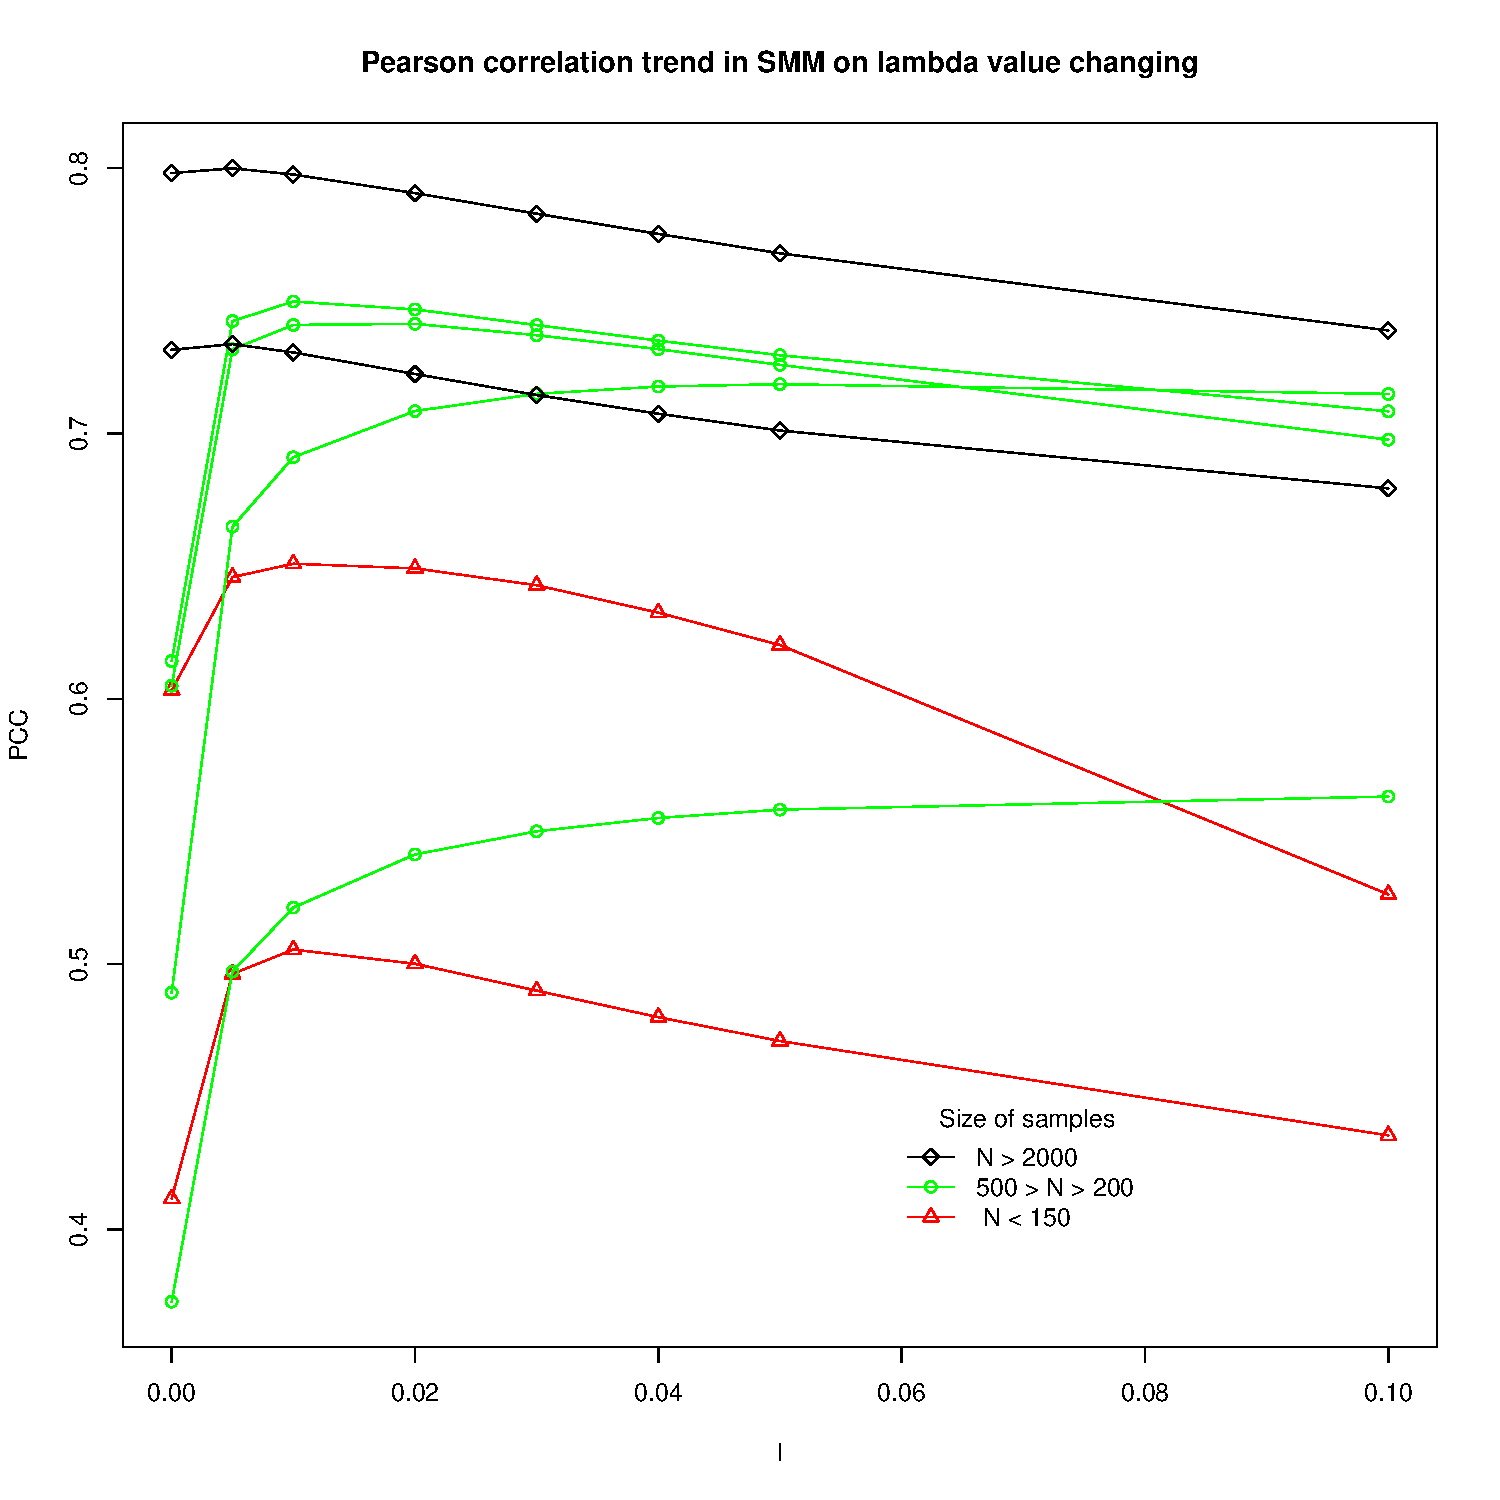
\includegraphics[width=9cm]{fig/smm_l005_ppc_size.pdf}}
\caption{Pearson's correlation coefficent  from the SMM Gradient Decent,of different sample using increasing values of $\lambda$. The sample were grouped by the size of the dataset. We can see how dataset of similar size show a similar trend of the Pearson correlation $\lambda$ depending.}
\label{fig:01}
\end{figure}

\begin{figure}[!tpb]
\centerline{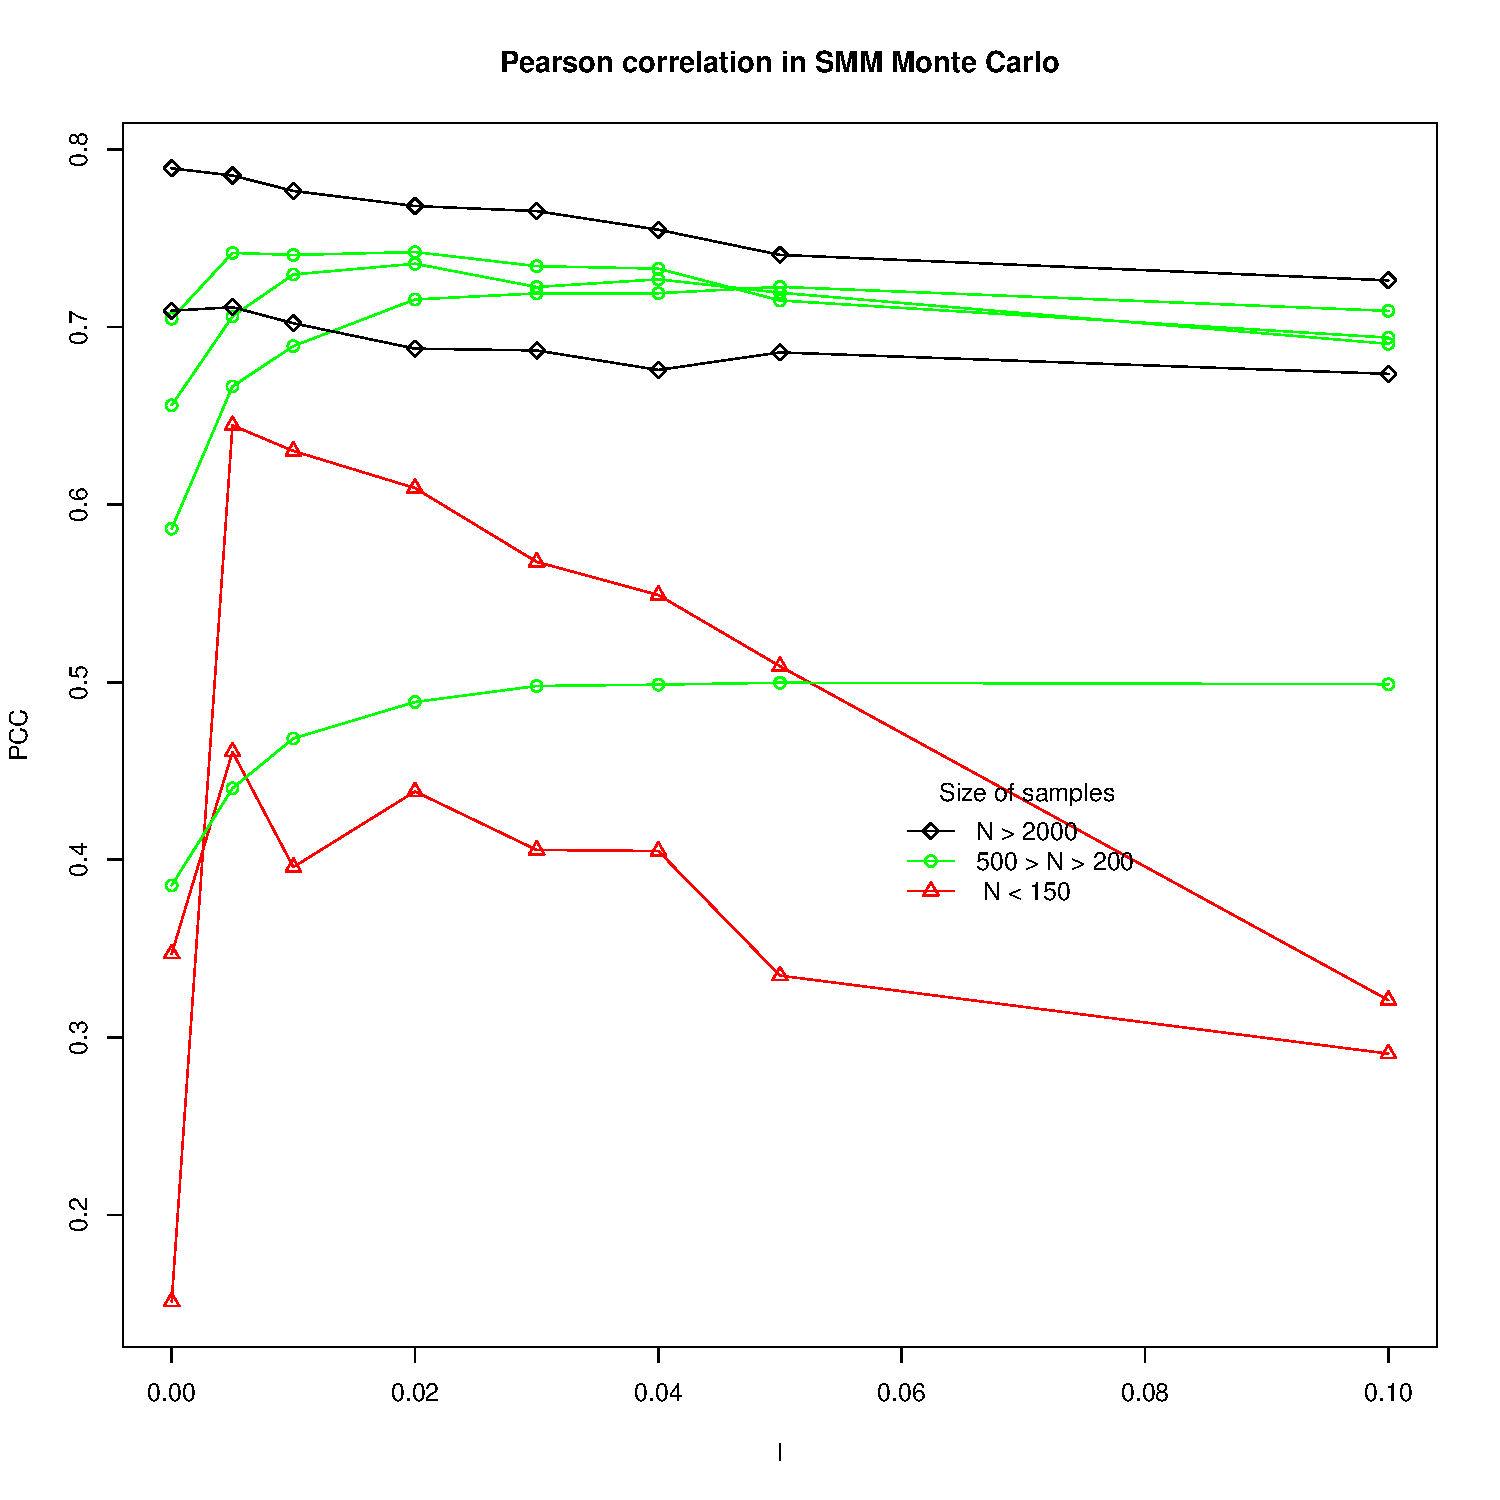
\includegraphics[width=9cm]{fig/smm_mc_l005_ppc_size.pdf}}
\caption{Pearson's correlation coefficent from the SMM Monte Calro, of different sample using increasing values of $\lambda$. The sample were grouped by the size of the dataset. We can see how dataset of similar size show a similar trend of the Pearson correlation $\lambda$ depending.}
\label{fig:02}
\end{figure}

\section*{Results}


Figure \ref{fig:01} shows the trend for Pearson's correlation coefficient (PCC, prediction accuracy) using different $\lambda$ values for various data sizes.


\begin{figure}[!tpb]
\centerline{\includegraphics[width=9cm]{fig/smm_error.png}}
\caption{Error trend for dataset of different size in function of the number of cycle of the SMM gradient decent algorithm}
\label{fig:03}
\end{figure}

\begin{figure}[!tpb]
\centerline{\includegraphics[width=9cm]{fig/smm_mc_error.png}}
\caption{Error trend for dataset of different size in function of the number of cycle of the SMM Monte Carlo algorithm}
\label{fig:04}
\end{figure}

\par As a general rule, as the data size gets larger the less important the effect of a non-zero $\lambda$ becomes. For large data sets a $\lambda$ value of zero seems to give the best results. A large dataset should average out the noise. Similar graph showing results from the Monte Carlo version says the same story (Figure \ref{fig:02}).
\par For the small datasets an optimal $\lambda$ value is  less than 0.01. Next we run the smm algorithms on a data from five different kinds of MHC molecules (with different data sizes) showing the error as a function of iterations. For the smm algorithm using gradient descent and 500 iterations, a default lambda value of 0.05 is used (Figure \ref{fig:03}). Similar chart is shown for the monte carlo version of the algorithm in Figure \ref{fig:04} showing 12000 iterations. The reason for showing different data sizes on the same chart is just for showing the trends in the two different algorithms. The gradient descent method converges much faster to an optimal value than the monte carlo method. The data sizes and percentage of number of binding peptides are shown in the parantheses right by the names of the lines representing each MHC molecule.


\begin{figure}[!tpb]
\centerline{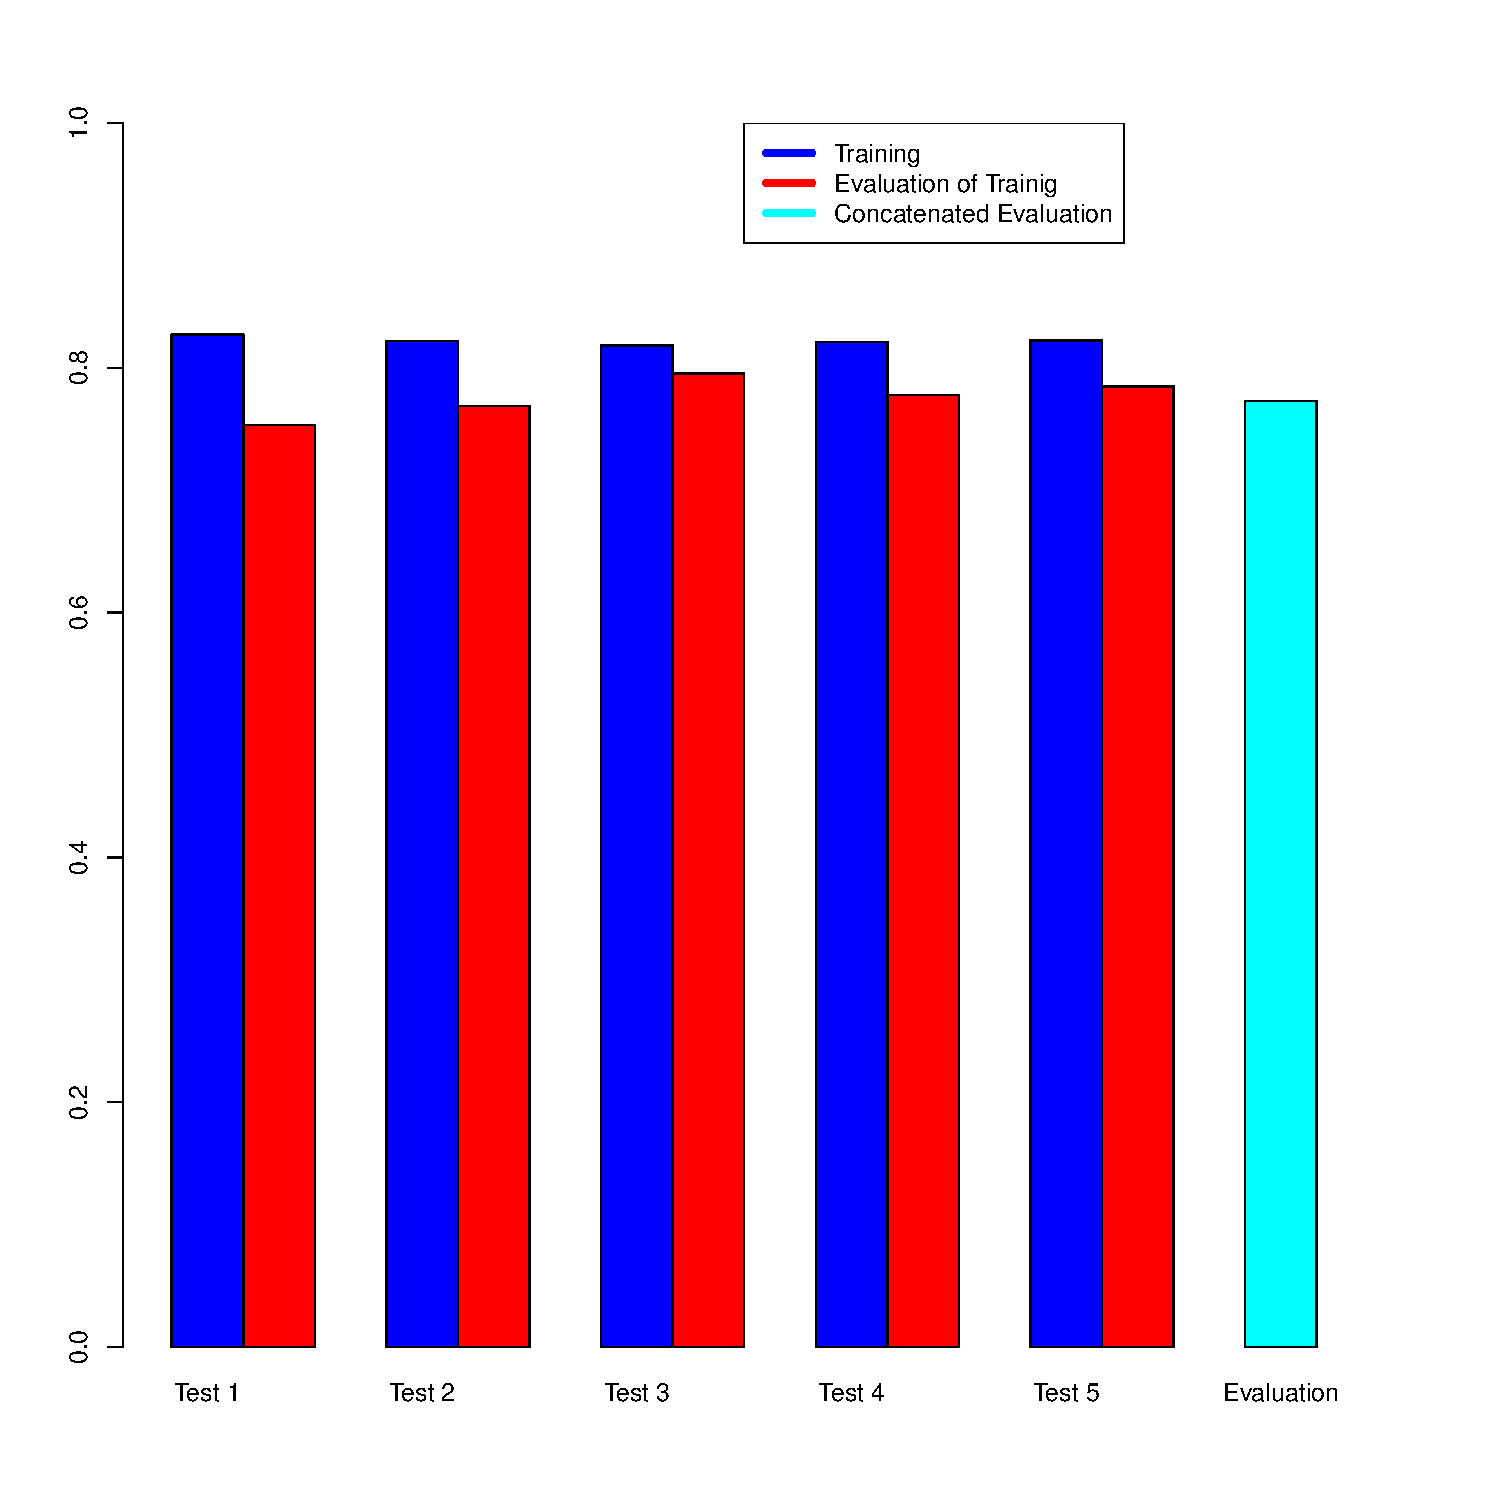
\includegraphics[width=9cm]{fig/barplot.pdf}}
\caption{Barplot showing the Pearson Correlation for each training set, for each evaluation on the test set and the correlation of the concatenate evaluation among the 5 test set}
\label{fig:05}
\end{figure}








%\bibliographystyle{natbib}
%\bibliographystyle{achemnat}
%\bibliographystyle{plainnat}
%\bibliographystyle{abbrv}
%\bibliographystyle{bioinformatics}

\bibliographystyle{abbrv}

\bibliography{algo}


\end{application}
\end{document}
